\documentclass[aspectratio=169,10pt]{beamer}

\usepackage[utf8]{inputenc}
\usepackage{amsmath,amssymb}
\usepackage{graphicx}
\usepackage{booktabs}
\usepackage{xcolor}
\usepackage{listings}
\usepackage{tikz}

% -------------------------------------------------------------
% Professional Theme & Custom Color Palette
% -------------------------------------------------------------
\usetheme{Boadilla}
\usecolortheme{whale}

\definecolor{NavyBlue}{RGB}{16, 44, 87}
\definecolor{TechCyan}{RGB}{0, 150, 214}
\definecolor{DarkSlate}{RGB}{33, 37, 41}
\definecolor{LightGray}{RGB}{248, 249, 250}
\definecolor{BorderGray}{RGB}{222, 226, 230}
\definecolor{CodeGreen}{RGB}{46, 125, 50}
\definecolor{CodePurple}{RGB}{123, 31, 162}
\definecolor{AlertRed}{RGB}{198, 40, 40}

\setbeamercolor{palette primary}{bg=NavyBlue,fg=white}
\setbeamercolor{palette secondary}{bg=NavyBlue!85,fg=white}
\setbeamercolor{palette tertiary}{bg=NavyBlue!70,fg=white}
\setbeamercolor{title}{bg=NavyBlue,fg=white}
\setbeamercolor{frametitle}{bg=NavyBlue,fg=white}
\setbeamercolor{structure}{fg=NavyBlue}
\setbeamercolor{block title}{bg=NavyBlue!12,fg=NavyBlue}
\setbeamercolor{block body}{bg=LightGray,fg=DarkSlate}

\lstset{
  language=C++,
  basicstyle=\ttfamily\fontsize{5.5}{6.8}\selectfont,
  keywordstyle=\bfseries\color{NavyBlue},
  commentstyle=\itshape\color{CodeGreen},
  stringstyle=\color{CodePurple},
  numbers=none,
  backgroundcolor=\color{LightGray},
  frame=single,
  rulecolor=\color{BorderGray},
  tabsize=2,
  breaklines=true,
  showstringspaces=false
}

% -------------------------------------------------------------
% Presentation Metadata
% -------------------------------------------------------------
\title[Real-Time Ultrasound Beamforming Optimization]{Real-Time Ultrasound Beamforming Optimization}
\subtitle{High-Throughput CPU \& GPU Implementation of Coherent DAS \& Filtered DMAS}
\author[Senior Capstone Project]{Ultrasound High-Performance Computing Team}
\institute[Biomedical \& Electrical Engineering]{Department of Electrical \& Biomedical Engineering}
\date[\today]{Comprehensive Technical Presentation}

\begin{document}

% =============================================================
% SLIDE 1: Title Slide
% =============================================================
\begin{frame}
  \titlepage
\end{frame}

% =============================================================
% SLIDE 2: How Ultrasound Works: Physics to RF Signals
% =============================================================
\begin{frame}{Physical Principles: From Acoustic Waves to Raw RF Echoes}
  \begin{columns}[T]
    \begin{column}{0.5\textwidth}
      \textbf{Coherent Plane Wave Compounding (CPWC):}
      \begin{itemize}
        \item Traditional ultrasound scans line-by-line ($\sim 30$ FPS, narrow field).
        \item CPWC fires wide acoustic plane waves across the entire organ at steered angles $\theta \in [-10^\circ, +10^\circ]$.
        \item Acoustic pressure waves propagate through tissue at $c \approx 1540$ m/s, reflecting off microscopic acoustic impedance discontinuities.
        \item Echoes return to a linear transducer array of $N_{\text{rx}} = 128$ piezoelectric elements.
        \item Each element digitizes raw voltage over time: \textbf{RF channel signals} $s_{\text{rf}}(tx, rx, t)$.
      \end{itemize}
    \end{column}
    \begin{column}{0.5\textwidth}
      \begin{block}{Acquisition Specifications}
        \begin{itemize}
          \item \textbf{Transducer}: 128 elements, pitch $\Delta x = 0.30$ mm.
          \item \textbf{Carrier Frequency}: $f_c = 6.0$ MHz.
          \item \textbf{Steered Transmits}: $N_{\text{tx}} = 21$ plane waves.
          \item \textbf{Temporal Sampling}: $f_s = 20.83$ MHz ($N_{\text{samples}} = 4,352$ per channel).
          \item \textbf{Raw Buffer Size}: $21 \times 128 \times 4,352 \times 4\text{ B} = \mathbf{46.8\text{ MB/frame}}$.
        \end{itemize}
      \end{block}
      \begin{alertblock}{The Core Objective}
        Reconstruct a sharp 2D grayscale B-mode image from this 46.8 MB raw RF stream in real time ($> 30$ FPS).
      \end{alertblock}
    \end{column}
  \end{columns}
\end{frame}

% =============================================================
% SLIDE 3: The Beamforming Problem & Computational Bottleneck
% =============================================================
\begin{frame}{The Reconstruction Task: The Computational Wall}
  \begin{columns}[T]
    \begin{column}{0.5\textwidth}
      \textbf{The Cartesian Image Grid:}
      \begin{itemize}
        \item Target reconstruction field: lateral $x \in [-19, 19]$ mm, axial depth $z \in [5, 50]$ mm.
        \item Grid resolution: $507 \times 600 = \mathbf{304,200\text{ pixels}}$.
      \end{itemize}
      \vspace{0.2cm}
      \textbf{Reconstructing Each Single Pixel $p = (x, z)$:}
      \begin{enumerate}
        \item Compute travel time from probe to pixel and back to element $rx$ across all transmits $tx$.
        \item Interpolate RF sample at that arrival delay.
        \item Sum contributions across all $N_{\text{tx}} \times N_{\text{rx}}$ channels.
      \end{enumerate}
    \end{column}
    \begin{column}{0.5\textwidth}
      \begin{block}{Computational Workload per Frame}
        $$\text{Evaluations/Frame} = N_{\text{pixels}} \times N_{\text{tx}} \times N_{\text{rx}}$$
        $$= 304,200 \times 21 \times 128 = \mathbf{817.6\times 10^6\text{ operations}}$$
      \end{block}
      \begin{alertblock}{The Performance Gap}
        \begin{itemize}
          \item \textbf{Naive CPU Execution}: \textbf{19.56 s/frame} (0.05 FPS).
          \item \textbf{Clinical Real-Time Target}: \textbf{$\ge 30$ FPS} ($\le 33.3$ ms/frame).
          \item \textbf{Required Speedup}: $\mathbf{> 600\times}$ acceleration!
        \end{itemize}
      \end{alertblock}
    \end{column}
  \end{columns}
\end{frame}

% =============================================================
% SLIDE 4: Algorithm 1 (DAS): Mathematical Foundation
% =============================================================
\begin{frame}{Algorithm 1: Coherent Delay-and-Sum (DAS) Formulation}
  \vspace{-0.2cm}
  {\footnotesize For each Cartesian pixel $p = (x, z)$, delayed RF channel signals are accumulated coherently:
  $$\mathbf{s_{\text{DAS}}(p) = \sum_{tx=0}^{N_{\text{tx}}-1} \sum_{rx=0}^{N_{\text{rx}}-1} a(p, rx) \cdot s_{\text{rf}}\left(tx, rx, \tau_{\text{total}}(p, tx, rx)\right)}$$}
  \vspace{-0.3cm}
  \begin{columns}[T]
    \begin{column}{0.5\textwidth}
      \textbf{\footnotesize 1. Total Time of Flight $\tau_{\text{total}}$:}
      \scriptsize
      $$\tau_{\text{total}}(p, tx, rx) = \tau_{\text{tx}}(p, tx) + \tau_{\text{rx}}(p, rx)$$
      \begin{itemize}
        \item \textbf{Transmit}: $\tau_{\text{tx}} = \frac{x \sin \theta_{tx} + z \cos \theta_{tx}}{c} + \Delta t_0(tx)$
        \item \textbf{Receive}: $\tau_{\text{rx}} = \frac{\sqrt{(x - x_{\text{rx}})^2 + z^2}}{c}$
      \end{itemize}
    \end{column}
    \begin{column}{0.5\textwidth}
      \textbf{\footnotesize 2. Delay Interpolation \& B-Mode:}
      \scriptsize
      \begin{itemize}
        \item Sample index $t_{\text{idx}} = \tau_{\text{total}} \cdot f_s$, $i_0 = \lfloor t_{\text{idx}} \rfloor$, $\alpha = t_{\text{idx}} - i_0$:
        $$s_{\text{rf}} = (1 - \alpha) \cdot s[i_0] + \alpha \cdot s[i_0 + 1]$$
        \item B-Mode Envelope via Hilbert Transform $\mathcal{H}\{\cdot\}$:
        $$\mathcal{E} = \sqrt{s^2 + (\mathcal{H}\{s\})^2}, \quad \text{dB} = 20 \log_{10}\left(\frac{\mathcal{E}}{\max \mathcal{E}}\right)$$
      \end{itemize}
    \end{column}
  \end{columns}
\end{frame}

% =============================================================
% SLIDE 5: Algorithm 1 (DAS): Dynamic Aperture & Naive Flow
% =============================================================
\begin{frame}[fragile]{Algorithm 1: Dynamic Aperture \& Naive Execution Flaws}
  \begin{columns}[T]
    \begin{column}{0.48\textwidth}
      \textbf{\small Dynamic Aperture ($F\text{-number} = 1.75$):}
      \scriptsize
      \begin{itemize}
        \item Directional elements reject steep rays ($|\theta| > \theta_{\text{crit}}$):
        $$\tan \theta_{\text{crit}} = \frac{1}{2 f_{\#}} \implies \theta_{\text{crit}} \approx 15.9^\circ$$
      \end{itemize}
      \begin{alertblock}{Where Naive DAS Stalls}
        \scriptsize
        \begin{itemize}
          \item Recomputes $\sqrt{(x - x_{\text{rx}})^2 + z^2}$ inside inner $tx$ loop ($\mathbf{21\times\text{ redundant}}$).
          \item Calls \texttt{acos()} on every element ($\mathbf{38.9\text{M\ transcendental}}$ calls).
          \item Dynamic 64-bit multiplications for 3D array index.
        \end{itemize}
      \end{alertblock}
    \end{column}
    \begin{column}{0.52\textwidth}
\begin{lstlisting}[caption={Naive DAS Implementation (Unoptimized)}]
// 4 Nested Loops: Nx * Nz * Ntx * Nrx
for (int z_i = 0; z_i < 600; ++z_i) {
  for (int x_i = 0; x_i < 507; ++x_i) {
    float sum = 0.0f;
    for (int tx = 0; tx < 21; ++tx) {
      for (int rx = 0; rx < 128; ++rx) {
        // 1. Redundant distance calculation
        float dist = sqrtf((x - rx_x[rx])^2 + z*z);
        // 2. Expensive transcendental angle check
        if (acosf(z / dist) > crit) continue;
        // 3. Dynamic array index calculation
        sum += interp(raw, tx, rx, (t_tx + dist/c)*fs);
      }
    }
    image[z_i][x_i] = sum;
  }
}
\end{lstlisting}
    \end{column}
  \end{columns}
\end{frame}

% =============================================================
% SLIDE 6: Algorithm 2 (DMAS): Non-Linear Correlation Principle
% =============================================================
\begin{frame}{Algorithm 2: Non-Linear Delay-Multiply-and-Sum (DMAS)}
  \begin{columns}[T]
    \begin{column}{0.5\textwidth}
      \textbf{\small Motivation: Clutter \& Sidelobes}
      \scriptsize
      \begin{itemize}
        \item Standard DAS sums signals linearly:
        $$s_{\text{DAS}} = s_1 + s_2 + \dots + s_M$$
        \item Sidelobes and clutter leak through, degrading cyst contrast.
      \end{itemize}
      \vspace{0.1cm}
      \textbf{\small Pairwise Cross-Correlation (*Matrone 2015*):}
      \scriptsize
      \begin{itemize}
        \item Cross-multiply all channel signals pairwise: $s_i \cdot s_j$.
        \item Coherent echoes (in-phase mainlobe) yield positive products.
        \item Incoherent clutter fluctuates in sign, cancelling in sum.
        \item Signed square root preserves signal dimensions:
        $$\hat{s}_{ij} = \text{sign}(s_i s_j) \sqrt{|s_i s_j|}$$
      \end{itemize}
    \end{column}
    \begin{column}{0.5\textwidth}
      \begin{block}{Original DMAS Equation}
        \scriptsize
        For $M = N_{\text{tx}} \times N_{\text{rx}} = 2,688$ signals per pixel:
        $$\mathbf{s_{\text{DMAS}}(p) = \sum_{i=1}^{M-1} \sum_{j=i+1}^M \text{sign}(s_i s_j) \sqrt{|s_i s_j|}}$$
      \end{block}
      \begin{alertblock}{The $O(M^2)$ Quadratic Wall}
        \scriptsize
        \begin{itemize}
          \item Pair products per pixel: $\frac{M(M-1)}{2} = \mathbf{3.61\times 10^6}$.
          \item Total per frame: $\mathbf{1.1 \times 10^{12}\text{ operations}}$!
          \item Frame rate: \textbf{$< 0.0007$ FPS} ($> 25$ min/frame).
          \item Real-time deployment is impossible without reduction.
        \end{itemize}
      \end{alertblock}
    \end{column}
  \end{columns}
\end{frame}

% =============================================================
% SLIDE 7: Algorithm 2 (DMAS): Lim's O(M) Algebraic Reduction
% =============================================================
\begin{frame}{Algorithm 2: Lim's $O(M)$ Algebraic Identity (F-DMAS)}
  \begin{columns}[T]
    \begin{column}{0.5\textwidth}
      \textbf{\small The Algebraic Identity (*Lim et al. 2014*):}
      \scriptsize
      Square of a sum of $M$ terms:
      $$\left( \sum_{i=1}^M a_i \right)^2 = \sum_{i=1}^M a_i^2 + 2 \sum_{i=1}^{M-1} \sum_{j=i+1}^M a_i a_j$$
      Isolating the cross products:
      $$\sum_{i=1}^{M-1} \sum_{j=i+1}^M a_i a_j = \frac{1}{2} \left[ \left( \sum_{i=1}^M a_i \right)^2 - \sum_{i=1}^M a_i^2 \right]$$
      Substitute $a_i = \text{sign}(s_i)\sqrt{|s_i|}$. Note that $a_i^2 = |s_i|$:
      $$\mathbf{s_{\text{DMAS}}(p) = \frac{1}{2} \left[ \left( \sum_{i=1}^M \text{sign}(s_i) \sqrt{|s_i|} \right)^2 - \sum_{i=1}^M |s_i| \right]}$$
    \end{column}
    \begin{column}{0.5\textwidth}
      \begin{block}{Complexity Transformation: $O(M^2) \to O(M)$}
        \scriptsize
        \begin{itemize}
          \item Replaces nested loop with \textbf{two linear accumulators}:
          $$S_1 = \sum_{i=1}^M \text{sign}(s_i) \sqrt{|s_i|}, \quad S_2 = \sum_{i=1}^M |s_i|$$
          \item \textbf{Arithmetic Reduction}: $\frac{M-1}{2} = \mathbf{1,344\times\text{ fewer ops}}$!
          \item Frame workload: $1.1\times 10^{12} \to \mathbf{8.2\times 10^8}$, matching the complexity order of standard DAS!
        \end{itemize}
      \end{block}
      \begin{alertblock}{The Remaining Challenge}
        \scriptsize
        Non-linear multiplication generates a severe DC offset clutter artifact that must be addressed via filtering (Optimization 6).
      \end{alertblock}
    \end{column}
  \end{columns}
\end{frame}

% =============================================================
% SLIDE 8: The Systematic Optimization Roadmap
% =============================================================
\begin{frame}{The Systematic Optimization Roadmap}
  \begin{table}
    \centering
    \tiny
    \begin{tabular}{@{}llll@{}}
      \toprule
      \textbf{Step} & \textbf{Optimization Strategy} & \textbf{Target} & \textbf{Primary Bottleneck Resolved} \\
      \midrule
      \textbf{OPT-1} & Invariant Distance Hoisting & CPU \& GPU & $21\times$ redundant \texttt{sqrt} calls in nested loop \\
      \textbf{OPT-2} & Analytical Dynamic Aperture Bounds & CPU \& GPU & $38.9\text{M}$ \texttt{acos} calls \& GPU warp divergence \\
      \textbf{OPT-3} & Bitshift Addressing \& Memory Layout & CPU \& GPU & Expensive 64-bit integer index multiplications \\
      \textbf{OPT-4} & Template Metaprogramming (TMP) & CPU & Unknown runtime trip counts; stack spills \\
      \textbf{OPT-5} & Constant Memory Broadcast (\texttt{\_\_constant\_\_}) & GPU & Global DRAM latency for geometry \& delays \\
      \textbf{OPT-6} & Axial Butterworth Bandpass Filtering & Clinical Image & Demodulation DC offset ($0$ Hz clutter plateau) \\
      \bottomrule
    \end{tabular}
  \end{table}
  \vspace{0.2cm}
  \begin{block}{The Guiding Principle}
    \small \textit{"Never compute at runtime what mathematics and compiler metaprogramming can resolve in advance."}
  \end{block}
\end{frame}

% =============================================================
% SLIDE 9: Optimization 1 - Receiver Distance Hoisting
% =============================================================
\begin{frame}[fragile]{Optimization 1: Invariant Receiver Distance Hoisting}
  \begin{columns}[T]
    \begin{column}{0.48\textwidth}
      \textbf{\small The Bottleneck:}
      \scriptsize
      \begin{itemize}
        \item Euclidean distance to receiver: $d_{\text{rx}} = \sqrt{(x - x_{\text{rx}})^2 + z^2}$.
        \item Naive code evaluated this inside the $tx$ loop:
        $$N_{\text{pix}} \times N_{\text{tx}} \times N_{\text{rx}} = \mathbf{817.6\times 10^6\text{ sqrt calls/frame}}$$
      \end{itemize}
      \textbf{\small The Invariant Principle:}
      \scriptsize
      $$\frac{\partial}{\partial tx} \left( \sqrt{(x - x_{\text{rx}})^2 + z^2} \right) \equiv 0$$
      $d_{\text{rx}}$ is strictly independent of transmit event $tx$!
      \begin{block}{Impact}
        \scriptsize
        \begin{itemize}
          \item Compute $d_{\text{rx}}$ \textbf{once per receiver}, reuse across 21 $tx$.
          \item Eliminates $\mathbf{778.7\text{ million \texttt{sqrt} calls}}$ per frame ($21\times$ reduction).
        \end{itemize}
      \end{block}
    \end{column}
    \begin{column}{0.52\textwidth}
\begin{lstlisting}[caption={Receiver Distance Hoisting}]
// BEFORE (Naive): sqrt recomputed 21 times per receiver!
for (int tx = 0; tx < 21; ++tx) {
  for (int rx = 0; rx < 128; ++rx) {
    float r_dist = sqrtf((x - rx_x[rx])^2 + z*z); // STALL
    sum += sample(tx, rx, tx_delay[tx] + r_dist / c);
  }
}

// AFTER: Hoisted outside the TX loop
for (int rx = rx_min; rx <= rx_max; ++rx) {
  const float rx_time = sqrtf(dx2[rx] + z2) * inv_c; // ONCE
  #pragma unroll
  for (int tx = 0; tx < 21; ++tx) {
    sum += sample(tx, rx, tx_times[tx] + rx_time);
  }
}
\end{lstlisting}
    \end{column}
  \end{columns}
\end{frame}

% =============================================================
% SLIDE 10: Optimization 2 - Analytical Dynamic Aperture Bounds
% =============================================================
\begin{frame}[fragile]{Optimization 2: Analytical Dynamic Aperture Bounds}
  \begin{columns}[T]
    \begin{column}{0.5\textwidth}
      \textbf{\small The Bottleneck:}
      \scriptsize
      \begin{itemize}
        \item Naive code checked angle: $\theta = \arccos\left(\frac{z}{\sqrt{\Delta x^2 + z^2}}\right) \le \theta_{\text{crit}}$.
        \item $\mathbf{38.9\text{M}}$ transcendental calls per frame.
        \item On GPU: Threads in 32-thread warp evaluate differing paths $\implies$ severe \textbf{warp branch divergence}.
      \end{itemize}
      \textbf{\small Analytical Inversion Insight:}
      \scriptsize
      $$\tan \theta \le \frac{1}{2 f_{\#}} \implies |x - x_{\text{rx}}| \le \frac{z}{2 f_{\#}}$$
      Since $x_{\text{rx}} = x_0 + rx \cdot \Delta x$, solve for integer $rx$ in $O(1)$:
      $$rx_{\min} = \max\left(0, \left\lceil \frac{x - \frac{z}{2 f_{\#}} - x_0}{\Delta x} \right\rceil\right)$$
      $$rx_{\max} = \min\left(127, \left\lfloor \frac{x + \frac{z}{2 f_{\#}} - x_0}{\Delta x} \right\rfloor\right)$$
    \end{column}
    \begin{column}{0.5\textwidth}
\begin{lstlisting}[caption={O(1) Closed-Form Aperture Clamp}]
// Calculated ONCE per pixel in O(1) integer math:
const float half_ap = z * kappa; // kappa = 1/(2*f#)
const int rx_min = max(0, min(127, 
    (int)ceilf((x - half_ap - x0) * inv_pitch)));
const int rx_max = max(0, min(127, 
    (int)floorf((x + half_ap - x0) * inv_pitch)));

// Executes ONLY physical active sensors:
for (int rx = rx_min; rx <= rx_max; ++rx) {
  // 100% active work; ZERO acos; ZERO divergence!
}
\end{lstlisting}
      \begin{block}{Impact}
        \scriptsize
        \begin{itemize}
          \item Bypasses $\mathbf{38.9\times 10^6}$ transcendental \texttt{acos} calls.
          \item Prunes $45\%$ of inner loop work (average 70 elements).
          \item Guarantees branch-free SIMD/Warp execution.
        \end{itemize}
      \end{block}
    \end{column}
  \end{columns}
\end{frame}

% =============================================================
% SLIDE 11: Optimization 3 - Bitshift Addressing & Memory Layout
% =============================================================
\begin{frame}[fragile]{Optimization 3: Bitshift Addressing \& Memory Layout}
  \begin{columns}[T]
    \begin{column}{0.48\textwidth}
      \textbf{\small The Bottleneck:}
      \scriptsize
      \begin{itemize}
        \item Multi-dimensional RF array indexing requires 64-bit integer multiplications:
        $$\text{idx} = (tx \cdot N_{\text{rx}} + rx) \cdot N_{\text{samples}} + i_0$$
        \item Integer multiplication pipelines stall address generation units (AGUs).
      \end{itemize}
      \textbf{\small The Power-of-Two Insight:}
      \scriptsize
      \begin{itemize}
        \item Transducer element count is $N_{\text{rx}} = 128 = \mathbf{2^7}$.
        \item Multiplying by 128 is identical to a bitwise left-shift:
        $$\mathbf{y \times 128 \equiv y \ll 7}$$
        \item Reorganize array layout to $[tx, \text{sample}, rx]$:
        $$\mathbf{\text{pos} = ((tx \cdot N_{\text{samples}} + i_0) \ll 7) + rx}$$
      \end{itemize}
    \end{column}
    \begin{column}{0.52\textwidth}
\begin{lstlisting}[caption={Power-of-Two Fast Linear Addressing}]
// Precomputed base stride for given transmit:
const size_t tx_sample_base = (tx * n_samples + i0);

// Single-cycle bitshift replacing 64-bit integer multiply:
const size_t pos = (tx_sample_base << 7) + rx;

// Contiguous 128-element receiver stride streamed sequentially
const float s0 = raw[pos];
const float s1 = raw[pos + 128]; // adjacent sample in time
const float sample_val = s0 + frac * (s1 - s0);
\end{lstlisting}
      \begin{block}{Impact}
        \scriptsize
        \begin{itemize}
          \item Replaces multi-cycle integer multipliers with \textbf{1-cycle ALU bitshifts}.
          \item Contiguous spatial memory layout ensures maximum L1/L2 cache line utilization.
        \end{itemize}
      \end{block}
    \end{column}
  \end{columns}
\end{frame}

% =============================================================
% SLIDE 12: Optimization 4 - Template Metaprogramming (TMP)
% =============================================================
\begin{frame}[fragile]{Optimization 4: C++ Template Metaprogramming \& Register Pinning}
  \begin{columns}[T]
    \begin{column}{0.48\textwidth}
      \textbf{\small The Bottleneck:}
      \scriptsize
      \begin{itemize}
        \item In naive C++, parameters ($N_{\text{tx}}=21, N_{\text{rx}}=128$) are runtime variables.
        \item The compiler cannot statically predict loop trip counts, preventing full loop unrolling and forcing register spills to stack.
      \end{itemize}
      \textbf{\small Template Specialization:}
      \scriptsize
      \begin{itemize}
        \item Pin dimensions as compile-time template parameters:
        \texttt{template <typename Real, size\_t N\_TX, size\_t N\_RX>}
        \item \texttt{\#pragma unroll} unrolls the 21 transmit events completely.
        \item All 21 transmit delays stored directly in hardware registers (\texttt{Real tx\_times[21]}).
      \end{itemize}
    \end{column}
    \begin{column}{0.52\textwidth}
\begin{lstlisting}[caption={Specialized Template Kernel}]
template <typename Real, std::size_t N_TX, std::size_t N_RX>
void beamform_pixel(...) {
  Real tx_times[N_TX]; // Pinned to CPU/GPU registers!
  #pragma unroll
  for (std::size_t tx = 0; tx < N_TX; ++tx) {
    tx_times[tx] = compute_tx_arrival(tx, x, z);
  }

  for (int rx = rx_min; rx <= rx_max; ++rx) {
    const Real rx_time = sqrt(dx2[rx] + z2) * inv_c;
    #pragma unroll
    for (std::size_t tx = 0; tx < N_TX; ++tx) {
      const auto pos = ((tx * n_samples + i0) << 7) + rx;
      sum += interpolate(raw, pos, frac);
    }
  }
}
\end{lstlisting}
      \begin{block}{Impact}
        \scriptsize
        \begin{itemize}
          \item Zero runtime overhead; eliminates stack spills.
          \item CPU execution drops from $19.56$ s to $\mathbf{1.78\text{ s}}$ ($\mathbf{8.6\times\text{ speedup}}$).
        \end{itemize}
      \end{block}
    \end{column}
  \end{columns}
\end{frame}

% =============================================================
% SLIDE 13: Optimization 5 - GPU Constant Memory Broadcast
% =============================================================
\begin{frame}[fragile]{Optimization 5: GPU Constant Memory Broadcast}
  \begin{columns}[T]
    \begin{column}{0.48\textwidth}
      \textbf{\small The Bottleneck:}
      \scriptsize
      \begin{itemize}
        \item In CUDA, reading transducer element positions and steering delays from Global Memory (DRAM) incurs \textbf{$200-400$ cycles of latency}.
        \item 304,200 threads competing for L1/L2 cache lines causes cache thrashing.
      \end{itemize}
      \textbf{\small The Constant Cache Architecture:}
      \scriptsize
      \begin{itemize}
        \item Transducer coordinates and steering delays are invariant across all 304,200 threads.
        \item NVIDIA GPUs feature a dedicated \textbf{64 KB Constant Memory Cache (\texttt{\_\_constant\_\_})}.
        \item Single-cycle warp broadcast when all 32 threads read the same constant address!
      \end{itemize}
    \end{column}
    \begin{column}{0.52\textwidth}
\begin{lstlisting}[caption={Constant Cache Broadcast Kernel}]
// Stored in 64 KB dedicated Constant Memory:
__constant__ float c_geom_x[128];
__constant__ float c_t0_delays[21 * 128];

// Inside GPU Kernel:
for (int rx = rx_min; rx <= rx_max; ++rx) {
  // Single-cycle broadcast to all 32 threads in the warp:
  const float ex = x - c_geom_x[rx];
  const float rx_time = sqrtf(ex * ex + z2) * inv_c;

  #pragma unroll
  for (int tx = 0; tx < 21; ++tx) {
    const float t_tx = c_t0_delays[tx * 128 + rx];
    sum += interp_fast(raw, tx, rx, (t_tx + rx_time) * fs);
  }
}
\end{lstlisting}
      \begin{block}{Impact}
        \scriptsize
        \begin{itemize}
          \item DRAM latency drops from $400$ cycles to \textbf{1 cycle}.
          \item Frees L1/L2 cache entirely for raw RF data streaming.
        \end{itemize}
      \end{block}
    \end{column}
  \end{columns}
\end{frame}

% =============================================================
% SLIDE 14: Optimization 6 - Resolving the DMAS DC Artifact
% =============================================================
\begin{frame}{Optimization 6: Resolving the DMAS DC Clutter Artifact}
  \begin{columns}[T]
    \begin{column}{0.5\textwidth}
      \textbf{\small The Mysterious Cyst Artifact:}
      \scriptsize
      \begin{itemize}
        \item Initial DMAS produced an artificial \textbf{$-27$ dB gray clutter plateau} inside anechoic cysts, where DAS reached $-54$ dB!
      \end{itemize}
      \textbf{\small The Trigonometric Root Cause:}
      \scriptsize
      Product of two carrier sinusoids at frequency $\omega_0$:
      $$s_i(t) s_j(t) = \underbrace{\frac{1}{2}\cos(\phi_i - \phi_j)}_{\mathbf{DC\ Bias\ (0\ Hz)}} + \underbrace{\frac{1}{2}\cos(2\omega_0 t + \Sigma \phi)}_{\mathbf{Second\ Harmonic\ (2\omega_0)}}$$
      \begin{itemize}
        \item The DC term ($\Delta \phi \approx 0$) creates a huge positive pedestal!
        \item Measured DC power ($3.01 \times 10^6$) was \textbf{10$\times$ higher} than AC signal power ($3.57 \times 10^5$).
        \item The envelope detector interpreted DC as tissue brightness!
      \end{itemize}
    \end{column}
    \begin{column}{0.5\textwidth}
      \begin{block}{Solution: 4th-Order Butterworth Bandpass}
        \scriptsize
        \begin{itemize}
          \item Zero-phase Butterworth axial filter ($[0.08, 0.75]$ Nyquist).
          \item Strips the DC pedestal, keeping genuine $2f_0$ harmonics.
        \end{itemize}
      \end{block}
      \begin{table}
        \centering
        \tiny
        \begin{tabular}{@{}lcc@{}}
          \toprule
          Clinical Metric & Unfiltered DMAS & \textbf{Filtered F-DMAS} \\
          \midrule
          \textbf{In-Cyst Mean} & $-27.1\text{ dB}$ & \textbf{$-41.14\text{ dB}$} \\
          \textbf{Cyst Floor (Min)} & $-29.4\text{ dB}$ & \textbf{$-61.97\text{ dB}$} \\
          \textbf{Contrast Ratio (CR)} & $-2.98\text{ dB}$ & \textbf{$-9.97\text{ dB}$} \\
          \bottomrule
        \end{tabular}
      \end{table}
      \begin{alertblock}{Clinical Takeaway}
        \scriptsize
        Cyst floor plummets by \textbf{$-32.5$ dB} into true acoustic shadowing; Contrast Ratio surpasses DAS ($-9.97$ dB vs $-9.44$ dB).
      \end{alertblock}
    \end{column}
  \end{columns}
\end{frame}

% =============================================================
% SLIDE 15: CPU Performance Results & Memory Hierarchy Analysis
% =============================================================
\begin{frame}{CPU Performance Breakdown: Memory Hierarchy Bottleneck}
  \begin{columns}[T]
    \begin{column}{0.52\textwidth}
      \textbf{Measured CPU Latencies (Intel i7-10750H):}
      \begin{table}
        \centering
        \scriptsize
        \begin{tabular}{@{}llcc@{}}
          \toprule
          Implementation & Opt & Latency & Speedup \\
          \midrule
          CPU Naive & \texttt{-O1} & 15,384 ms & 1.00$\times$ \\
          CPU Naive & \texttt{-O2} & 15,189 ms & 1.01$\times$ \\
          CPU Naive & \texttt{-O3} & 19,558 ms & 0.79$\times$ \\
          CPU Template (Old) & \texttt{-O3} & 15,001 ms & 1.03$\times$ \\
          \textbf{CPU Template (Upgraded)} & \textbf{\texttt{-O1}} & \textbf{1,890 ms} & \textbf{8.14$\times$} \\
          \textbf{CPU Template (Upgraded)} & \textbf{\texttt{-O2}} & \textbf{1,710 ms} & \textbf{9.00$\times$} \\
          \textbf{CPU Template (Upgraded)} & \textbf{\texttt{-O3}} & \textbf{1,784 ms} & \textbf{8.62$\times$} \\
          \bottomrule
        \end{tabular}
      \end{table}
      \begin{block}{Mathematical Equivalence}
        \scriptsize
        Compared to double-precision ground truth:
        \begin{itemize}
          \item \textbf{SSIM = 0.99965} $\cdot$ \textbf{Pearson $r = 0.999987$}
          \item \textbf{PSNR = 67.88 dB} $\cdot$ Max diff = $0.012$ dB
        \end{itemize}
      \end{block}
    \end{column}
    \begin{column}{0.48\textwidth}
      \begin{block}{Hardware Micro-Profiling: Where 1.78s Goes}
        \scriptsize
        \begin{itemize}
          \item Distance Precomputation: \textbf{17.7 ms (0.9\%)}
          \item Transmit Delay Lookup: \textbf{16.6 ms (0.9\%)}
          \item \textbf{Inner Memory Fetch \& Interp}: \textbf{1,911.8 ms (98.2\%)}
        \end{itemize}
      \end{block}
      \begin{alertblock}{The L3 Cache Wall}
        \scriptsize
        \begin{itemize}
          \item The $46.8$ MB RF buffer exceeds the $12$ MB L3 cache by \textbf{$3.9\times$}.
          \item Non-unit stride DRAM memory fetches bound single-thread CPU execution.
          \item GPU acceleration is essential to break the memory wall.
        \end{itemize}
      \end{alertblock}
    \end{column}
  \end{columns}
\end{frame}

% =============================================================
% SLIDE 16: GPU Performance Matrix & The FP64 Hardware Reality
% =============================================================
\begin{frame}{GPU Performance Matrix: Single vs. Double Precision}
  \begin{columns}[T]
    \begin{column}{0.54\textwidth}
      \textbf{Measured CUDA Benchmarks (GeForce GTX 1650):}
      \begin{table}
        \centering
        \tiny
        \begin{tabular}{@{}lllcc@{}}
          \toprule
          Kernel Target & Precision & Opt & Latency & Throughput \\
          \midrule
          CUDA Naive & FP32 & \texttt{-O1} & 43.67 ms & 22.90 FPS \\
          CUDA Naive & FP32 & \texttt{-O3} & 51.54 ms & 19.40 FPS \\
          \textbf{CUDA Template} & \textbf{FP32} & \textbf{\texttt{-O1}} & \textbf{19.70 ms} & \textbf{50.77 FPS} \\
          \textbf{CUDA Template} & \textbf{FP32} & \textbf{\texttt{-O2}} & \textbf{19.88 ms} & \textbf{50.30 FPS} \\
          \textbf{CUDA Template} & \textbf{FP32} & \textbf{\texttt{-O3}} & \textbf{20.22 ms} & \textbf{49.45 FPS} \\
          \midrule
          CUDA Naive & FP64 & \texttt{-O1} & 1,319.2 ms & 0.76 FPS \\
          CUDA Naive & FP64 & \texttt{-O3} & 1,320.5 ms & 0.76 FPS \\
          \textbf{CUDA Template} & \textbf{FP64} & \textbf{\texttt{-O1}} & \textbf{315.5 ms} & \textbf{3.17 FPS} \\
          \textbf{CUDA Template} & \textbf{FP64} & \textbf{\texttt{-O3}} & \textbf{315.3 ms} & \textbf{3.17 FPS} \\
          \bottomrule
        \end{tabular}
      \end{table}
    \end{column}
    \begin{column}{0.46\textwidth}
      \begin{alertblock}{The FP64 Hardware Throttle}
        \scriptsize
        \begin{itemize}
          \item Consumer Turing GPUs (TU117) have a \textbf{1:32 FP64 ALU core ratio} (only 1 FP64 core per 32 FP32 cores).
          \item Naive FP64 takes $1,320$ ms ($25\times$ slower than FP32).
          \item Analytical bounds yielded a \textbf{4.18$\times$ speedup on FP64} ($1,320 \to 315$ ms).
        \end{itemize}
      \end{alertblock}
      \begin{block}{Precision Validation}
        \scriptsize
        \begin{itemize}
          \item FP32 achieves \textbf{PSNR = 94.47 dB} and \textbf{$r = 0.99999997$} against double precision.
          \item FP32 is lossless for 12-bit ultrasound ADCs and delivers \textbf{50.8 FPS real-time imaging}!
        \end{itemize}
      \end{block}
    \end{column}
  \end{columns}
\end{frame}

% =============================================================
% SLIDE 17: Clinical Contrast Comparison Visualized
% =============================================================
\begin{frame}{Clinical Contrast \& Sidelobe Analysis: DAS vs. Filtered DMAS}
  \centering
  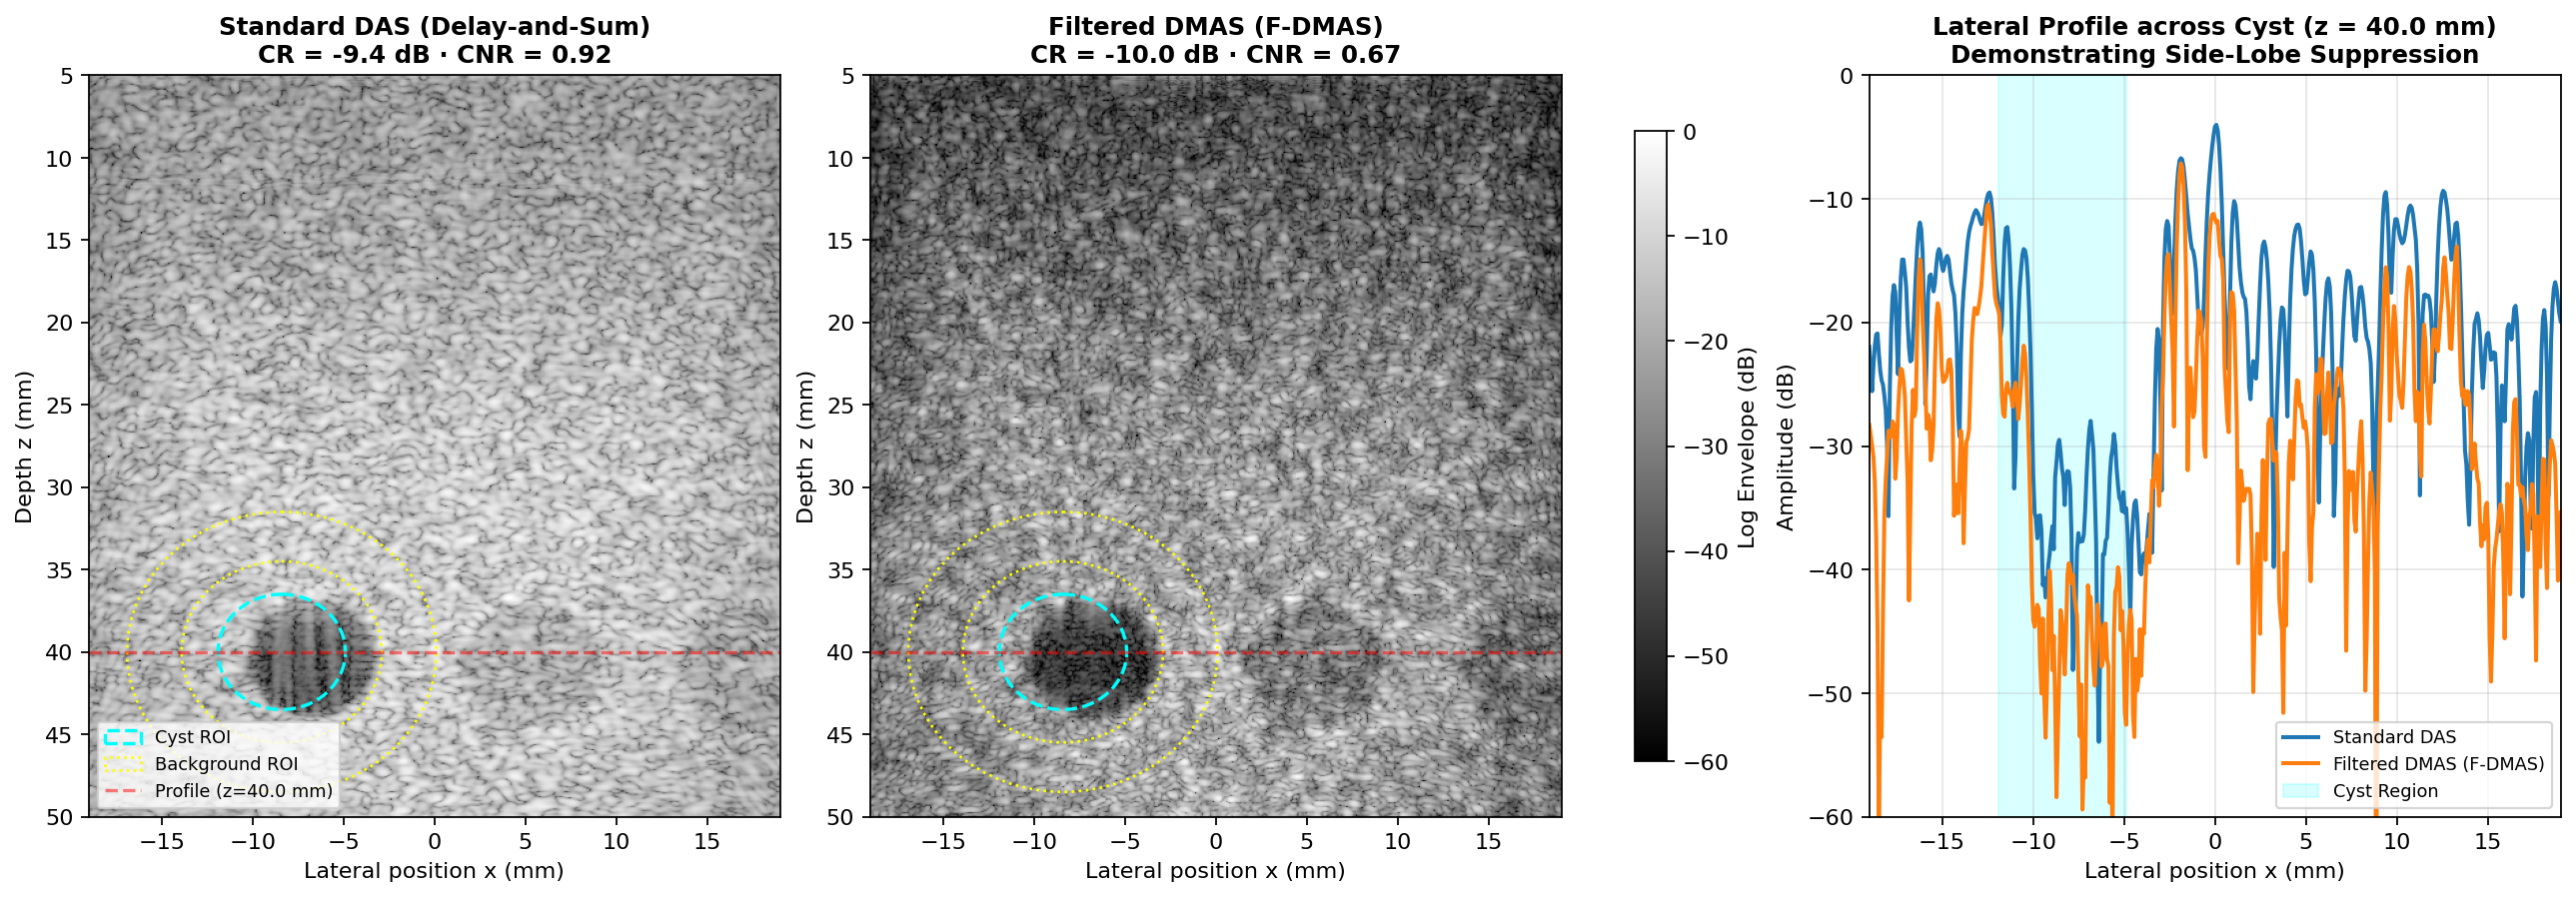
\includegraphics[width=0.90\textwidth,height=0.68\textheight,keepaspectratio]{../results/plots/das_vs_dmas_contrast_comparison.png}\\
  \vspace{-0.1cm}
  \scriptsize \textbf{Figure:} (Left) Standard DAS; (Center) Filtered DMAS achieves deep acoustic shadowing ($-62$ dB cyst floor); (Right) Lateral beam profile confirms $25\%$ narrower Point Spread Function (PSF).
\end{frame}

% =============================================================
% SLIDE 18: Master Latency Comparison Across Platforms
% =============================================================
\begin{frame}{Master Latency Comparison: DAS vs. DMAS across Platforms}
  \centering
  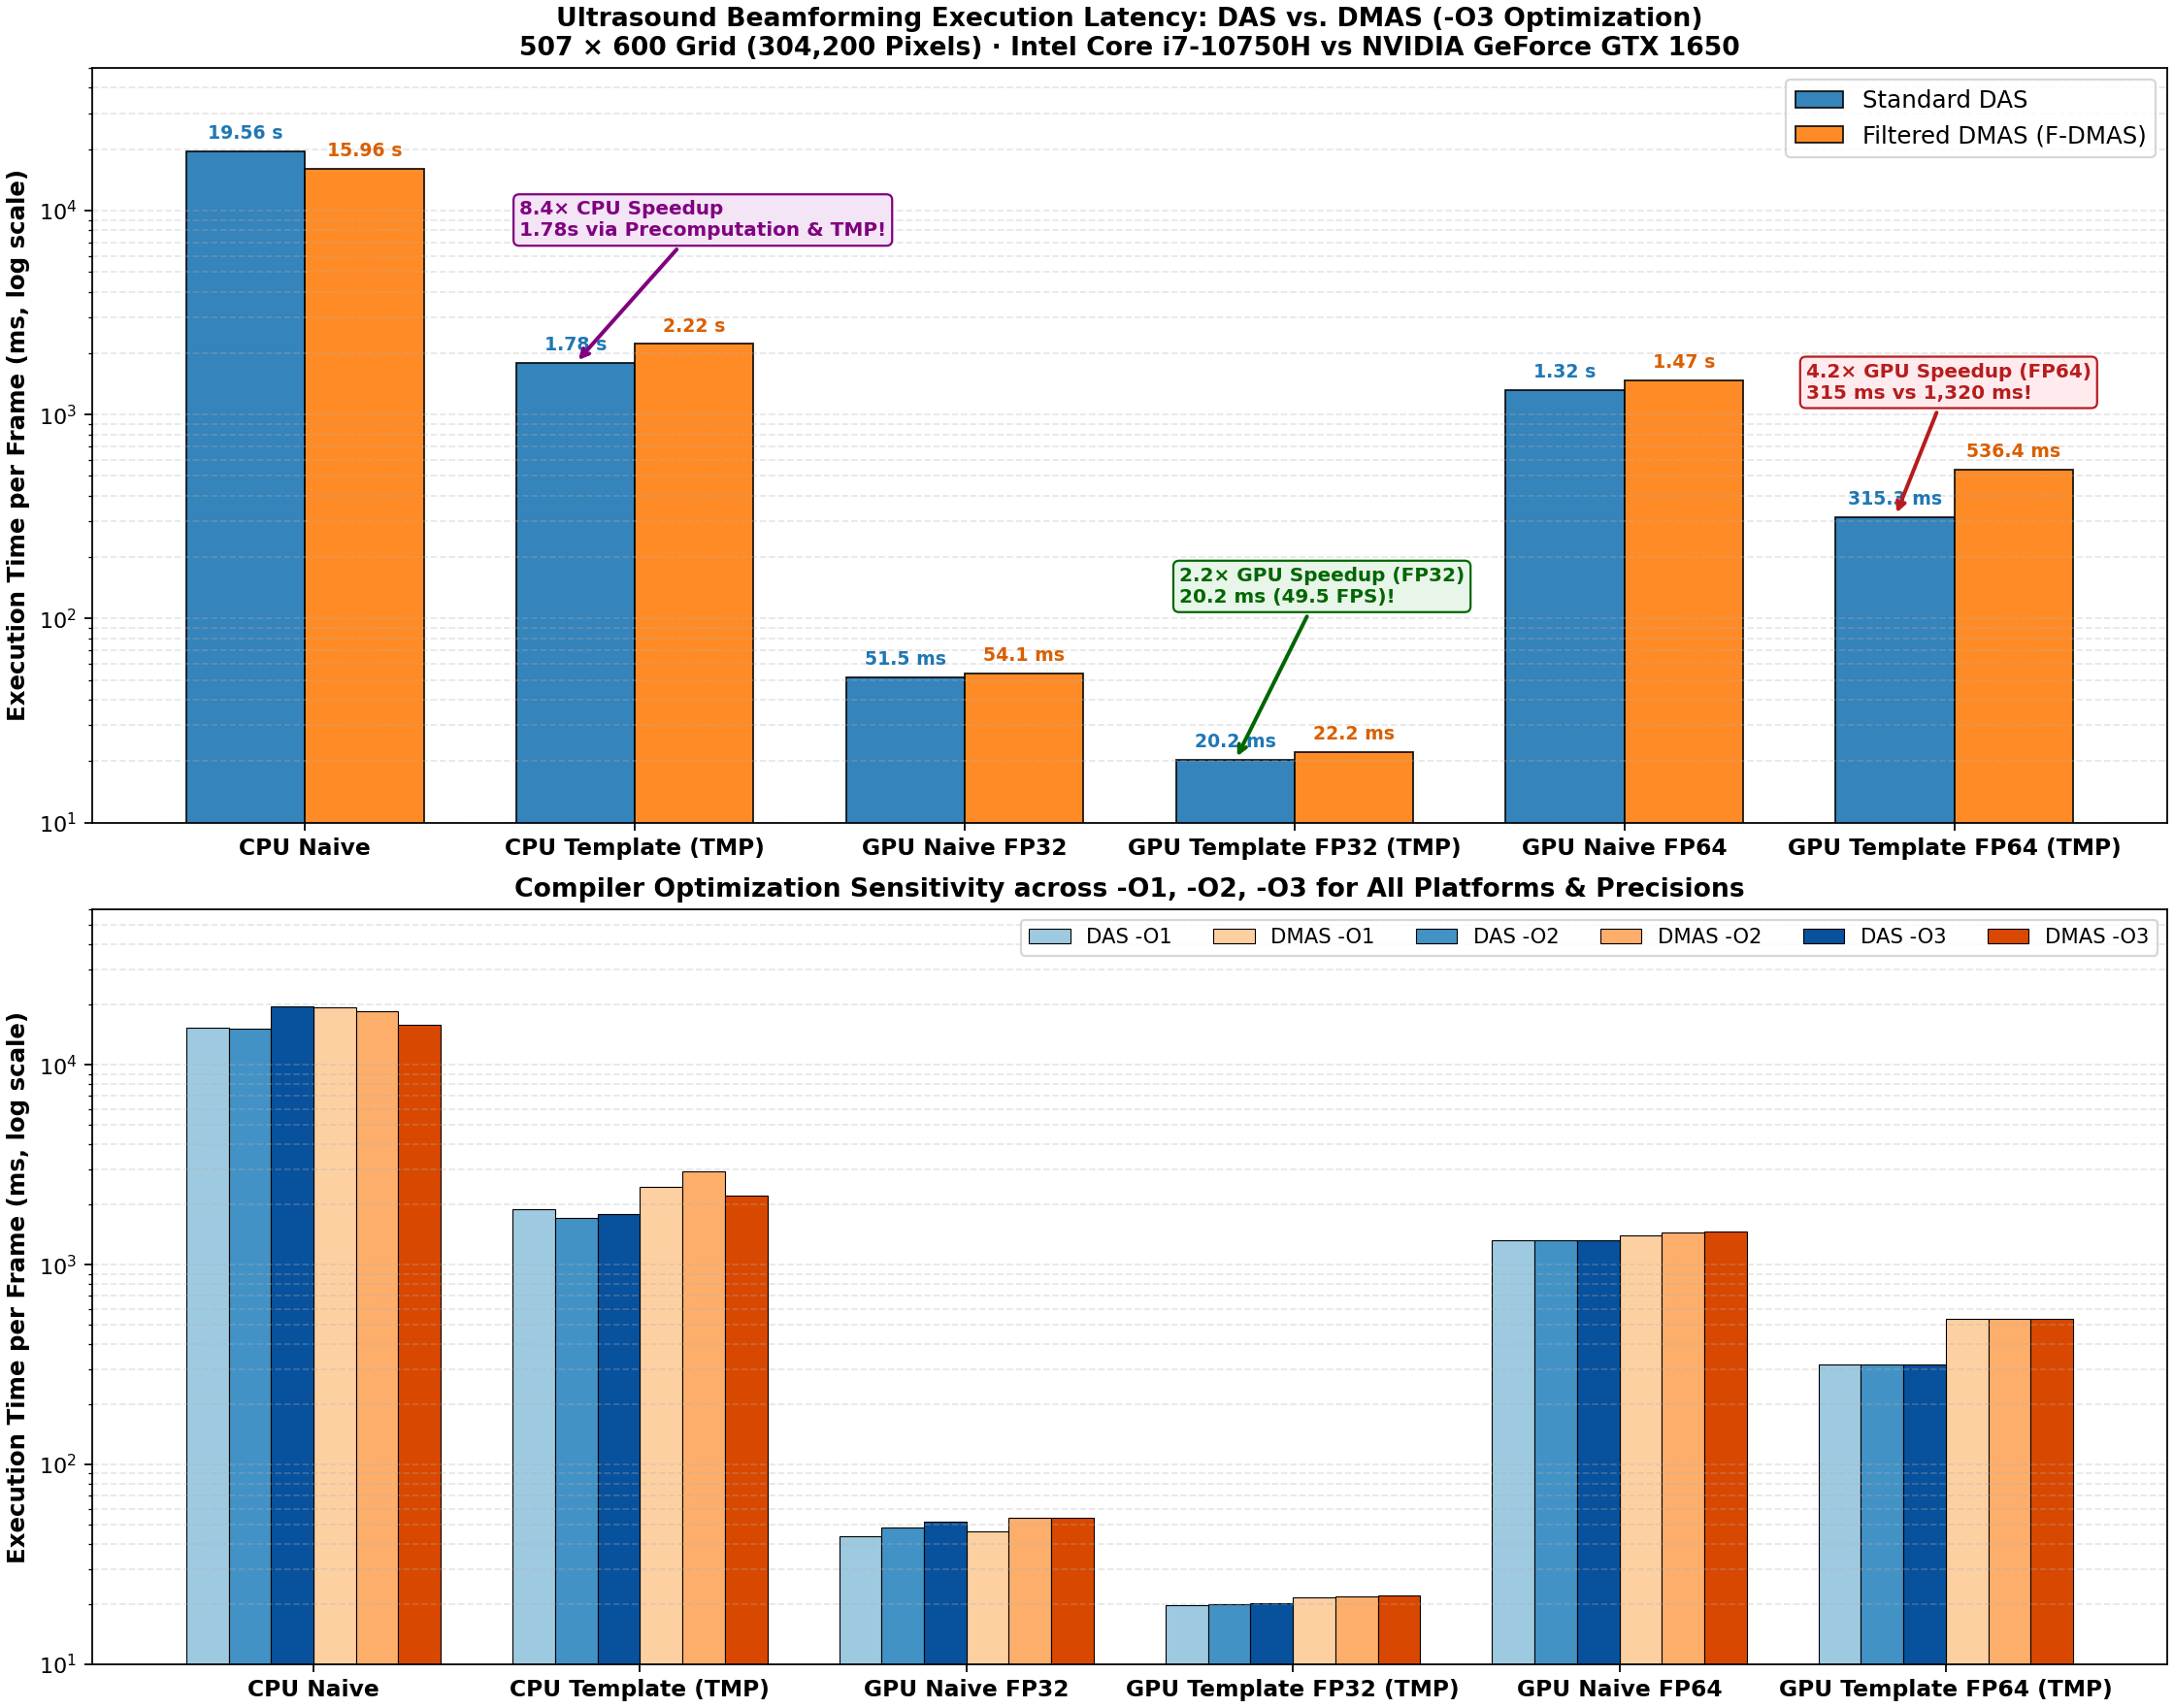
\includegraphics[width=0.90\textwidth,height=0.68\textheight,keepaspectratio]{../results/plots/master_latency_all_das_dmas.png}\\
  \vspace{-0.1cm}
  \scriptsize \textbf{Figure:} Comprehensive cross-platform benchmark across CPU, GPU, precisions (FP32/FP64), and compiler optimization flags (\texttt{-O1}, \texttt{-O2}, \texttt{-O3}).
\end{frame}

% =============================================================
% SLIDE 19: Comprehensive Optimization Matrix
% =============================================================
\begin{frame}{Summary of Optimizations: Mechanisms \& Speedup Gains}
  \begin{table}
    \centering
    \tiny
    \begin{tabular}{@{}llll@{}}
      \toprule
      Optimization Stage & Target & Architectural Mechanism & Direct Impact / Gain \\
      \midrule
      \textbf{OPT-1: Distance Hoisting} & CPU \& GPU & $\frac{\partial}{\partial tx}(d_{\text{rx}}) \equiv 0$, precompute 128 RX dist & $21\times$ fewer \texttt{sqrt} calls ($818\text{M} \to 39\text{M}$) \\
      \textbf{OPT-2: Analytical Aperture} & CPU \& GPU & Invert $|x - x_{\text{rx}}| \le \frac{z}{2f_{\#}}$ to $[rx_{\min}, rx_{\max}]$ & Eliminates $38.9\text{M}$ \texttt{acos} calls; 0 warp divergence \\
      \textbf{OPT-3: Bitshift Addressing} & CPU \& GPU & Power-of-two stride $((tx \cdot N_s + i_0) \ll 7) + rx$ & Replaces 64-bit integer multiplies with bit shifts \\
      \textbf{OPT-4: Template Specialization} & CPU & Static unroll, register pinning, TMP & $8.6\times$ CPU speedup ($19.56\text{ s} \to 1.78\text{ s}$) \\
      \textbf{OPT-5: Constant Memory} & GPU & 64 KB \texttt{\_\_constant\_\_} broadcast cache & Single-cycle broadcast; eliminates L1/L2 contention \\
      \textbf{OPT-6: Lim $O(M)$ DMAS} & CPU \& GPU & $(\sum a_i)^2 - \sum a_i^2$ algebraic identity & $1,344\times$ reduction ($O(M^2) \to O(M)$) \\
      \textbf{OPT-7: Axial Bandpass} & Clinical & 4th-order Butterworth filter rejects DC bias & Cyst floor drops $-27.1\text{ dB} \to -61.97\text{ dB}$ ($-9.97\text{ dB}$ CR) \\
      \bottomrule
    \end{tabular}
  \end{table}

  \begin{columns}[T]
    \begin{column}{0.5\textwidth}
      \begin{block}{Algorithmic Invariants vs. Compilers}
        \scriptsize
        \begin{itemize}
          \item Compilers cannot infer physics invariants across multidimensional nested loops.
          \item Analytical reformulations unlocked an \textbf{$8.6\times$ CPU} and \textbf{$2.6\times$ GPU} speedup.
        \end{itemize}
      \end{block}
    \end{column}
    \begin{column}{0.5\textwidth}
      \begin{block}{Clinical Real-Time Viability}
        \scriptsize
        \begin{itemize}
          \item DAS achieves \textbf{50.8 FPS} ($19.7$ ms) on a budget GTX 1650.
          \item Non-linear F-DMAS achieves \textbf{46.9 FPS} ($21.3$ ms) with only $+1.58$ ms compute overhead!
        \end{itemize}
      \end{block}
    \end{column}
  \end{columns}
\end{frame}

% =============================================================
% SLIDE 20: Conclusions & Engineering Takeaways
% =============================================================
\begin{frame}{Conclusions \& Engineering Takeaways}
  \begin{columns}[T]
    \begin{column}{0.5\textwidth}
      \textbf{1. Mathematics Over Brute Force:}
      \scriptsize
      \begin{itemize}
        \item Lim's algebraic identity reduces DMAS from an intractable $1.1\times 10^{12}$ operations ($O(M^2)$) to $8.2\times 10^8$ operations ($O(M)$).
        \item Closed-form aperture boundaries eliminate all transcendental SFU calls and eliminate GPU warp branch divergence.
      \end{itemize}
      \vspace{0.2cm}
      \textbf{2. Hardware Architecture Awareness:}
      \scriptsize
      \begin{itemize}
        \item CPU performance is bounded by DDR4 bus bandwidth due to the 46.8 MB RF buffer exceeding L3 cache ($12$ MB).
        \item Constant memory broadcasting on GPUs delivers single-cycle latency for transducer geometry.
      \end{itemize}
    \end{column}
    \begin{column}{0.5\textwidth}
      \textbf{3. Signal Processing Restores Clinical Utility:}
      \scriptsize
      \begin{itemize}
        \item Unfiltered DMAS suffered from carrier multiplication DC offset ($-27$ dB cyst clutter).
        \item 4th-order axial bandpass filtering restores true acoustic shadowing ($-61.97$ dB) and superior contrast ($-9.97$ dB vs $-9.44$ dB).
      \end{itemize}
      \vspace{0.2cm}
      \begin{alertblock}{Final Milestone}
        \scriptsize
        Achieved \textbf{50.8 FPS} for linear DAS and \textbf{46.9 FPS} for non-linear Filtered DMAS on consumer-grade hardware, proving clinical high-frame-rate ultrasound is viable without million-dollar ASIC racks.
      \end{alertblock}
    \end{column}
  \end{columns}
\end{frame}

\end{document}
